\documentclass[12pt, aspectratio=169]{beamer}
\usepackage{
    hyperref,
    graphicx,
    transparent,
    siunitx,
    pgfpages,
    caption,
    booktabs,
    multirow,
    bm,
    standalone,
    tikz,
    comment,
    xcolor,
    svg,
}
\usepackage[hang,flushmargin]{footmisc}
\setbeameroption{hide notes}
% \setbeameroption{show only notes}
% \setbeameroption{show notes on second screen}
\setbeamertemplate{note page}[plain]
% \setbeamercovered{transparent}

% get rid of junk
\usetheme{default}
\usecolortheme{orchid}
\beamertemplatenavigationsymbolsempty
\hypersetup{pdfpagemode=UseNone} % don't show bookmarks on initial view

% named colors
\definecolor{offwhite}{RGB}{249,242,215}
\definecolor{foreground}{RGB}{255,255,255}
\definecolor{background}{RGB}{24,24,24}
\definecolor{title}{RGB}{107,174,214}
\definecolor{gray}{RGB}{155,155,155}
\definecolor{subtitle}{RGB}{102,255,204}
\definecolor{hilight}{RGB}{102,255,204}
\definecolor{vhilight}{RGB}{255,111,207}
\definecolor{lolight}{RGB}{155,155,155}
%\definecolor{green}{RGB}{125,250,125}

% use those colors
\setbeamercolor{titlelike}{fg=title}
\setbeamercolor{subtitle}{fg=subtitle}
\setbeamercolor{institute}{fg=gray}
\setbeamercolor{normal text}{fg=foreground,bg=background}
\setbeamercolor{item}{fg=foreground} % color of bullets
\setbeamercolor{subitem}{fg=foreground}
\setbeamercolor{itemize/enumerate subbody}{fg=foreground}
\setbeamercolor{section in toc}{fg=title}
\setbeamercolor{alerted text}{fg=title}

\setbeamertemplate{itemize subitem}{{\textendash}}
\setbeamerfont{itemize/enumerate subbody}{size=\footnotesize}
\setbeamerfont{itemize/enumerate subitem}{size=\footnotesize}

\addtobeamertemplate{block alerted begin}{%
  \setbeamercolor{alerted text}{fg=red}%
}{}
\addtobeamertemplate{block example begin}{%
  \setbeamercolor{alerted text}{fg=green}%
}{}

% add a bit of space at the top of the notes page
\addtobeamertemplate{note page}{\setlength{\parskip}{12pt}}

% a few macros
\setbeamertemplate{description item}{
    \hfill\alert{\textbf{\insertdescriptionitem}}
}
\setbeamertemplate{itemize items}[circle]

\AtBeginSection[]{
    \begin{frame}
        \vfill
        \centering
        \Huge\color{title}\insertsectionhead
        \vfill
    \end{frame}
}

\newcommand\blfootnote[1]{%
    \begingroup
    \renewcommand\thefootnote{}\footnote{\tiny \color{lolight} #1}%
    \huge%
    \addtocounter{footnote}{-1}%
    \endgroup
}

% math macros
\renewcommand{\d}[1]{\mathsf{d}#1}
\newcommand{\diff}[2]{\frac{\mathsf{d} #1}{\mathsf{d} #2}}
\newcommand{\pdiff}[2]{\frac{\partial #1}{\partial #2}}
\newcommand{\Diff}[2]{\frac{\mathsf{D} #1}{\mathsf{D} #2}}
\renewcommand\vec{\bm}
\newcommand{\uvec}[1]{\vec{\hat{#1}}}
\newcommand{\grad}{\vec{\nabla}}
\newcommand{\prandtl}{\ensuremath{\mathsf{Pr}}}
\newcommand{\rayleigh}{\ensuremath{\mathsf{Ra}}}

% text macros
\newcommand{\rb}{Rayleigh-B\'{e}nard}

\title{
    How should we represent unresolved processes in climate models?
}
\subtitle{A data-driven approach for Rayleigh-Bénard convection}
\author{Thomas Schanzer}
\institute{
    School of Physics and Climate Change Research Centre
}
\date{Tuesday 14 November 2023}


\begin{document}

\begin{frame}
\maketitle
\end{frame}

\begin{frame}
    \centering
    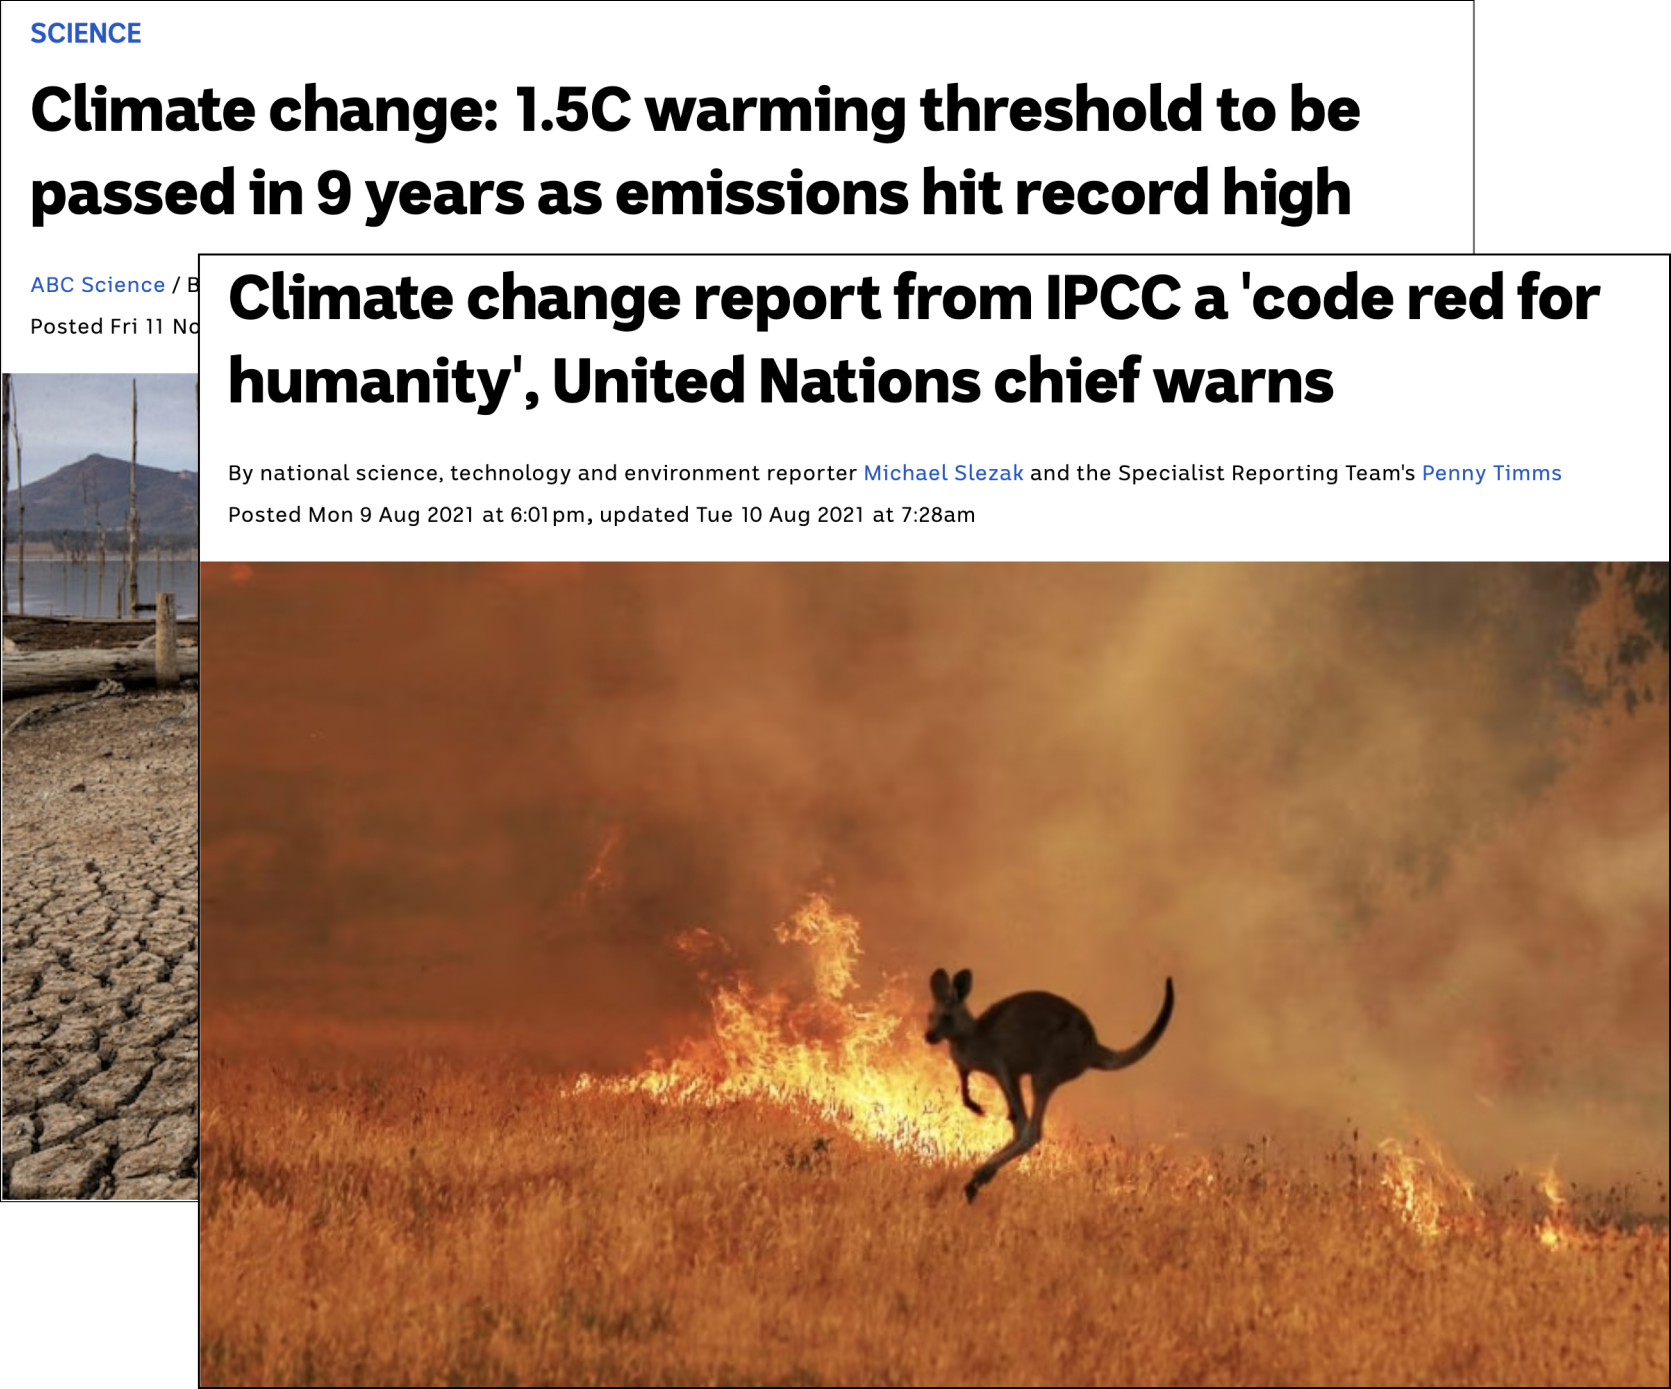
\includegraphics[height=0.99\textheight]{figures/news.png}
\end{frame}

\begin{frame}
    \centering
    \includegraphics[width=\linewidth]{figures/resolution1.pdf}
\end{frame}

\begin{frame}
    \centering
    \includegraphics[width=\linewidth]{figures/resolution2.pdf}
\end{frame}

\begin{frame}
    \centering
    \includegraphics[width=\linewidth]{figures/resolution3.pdf}
\end{frame}

\begin{frame}
    \centering
    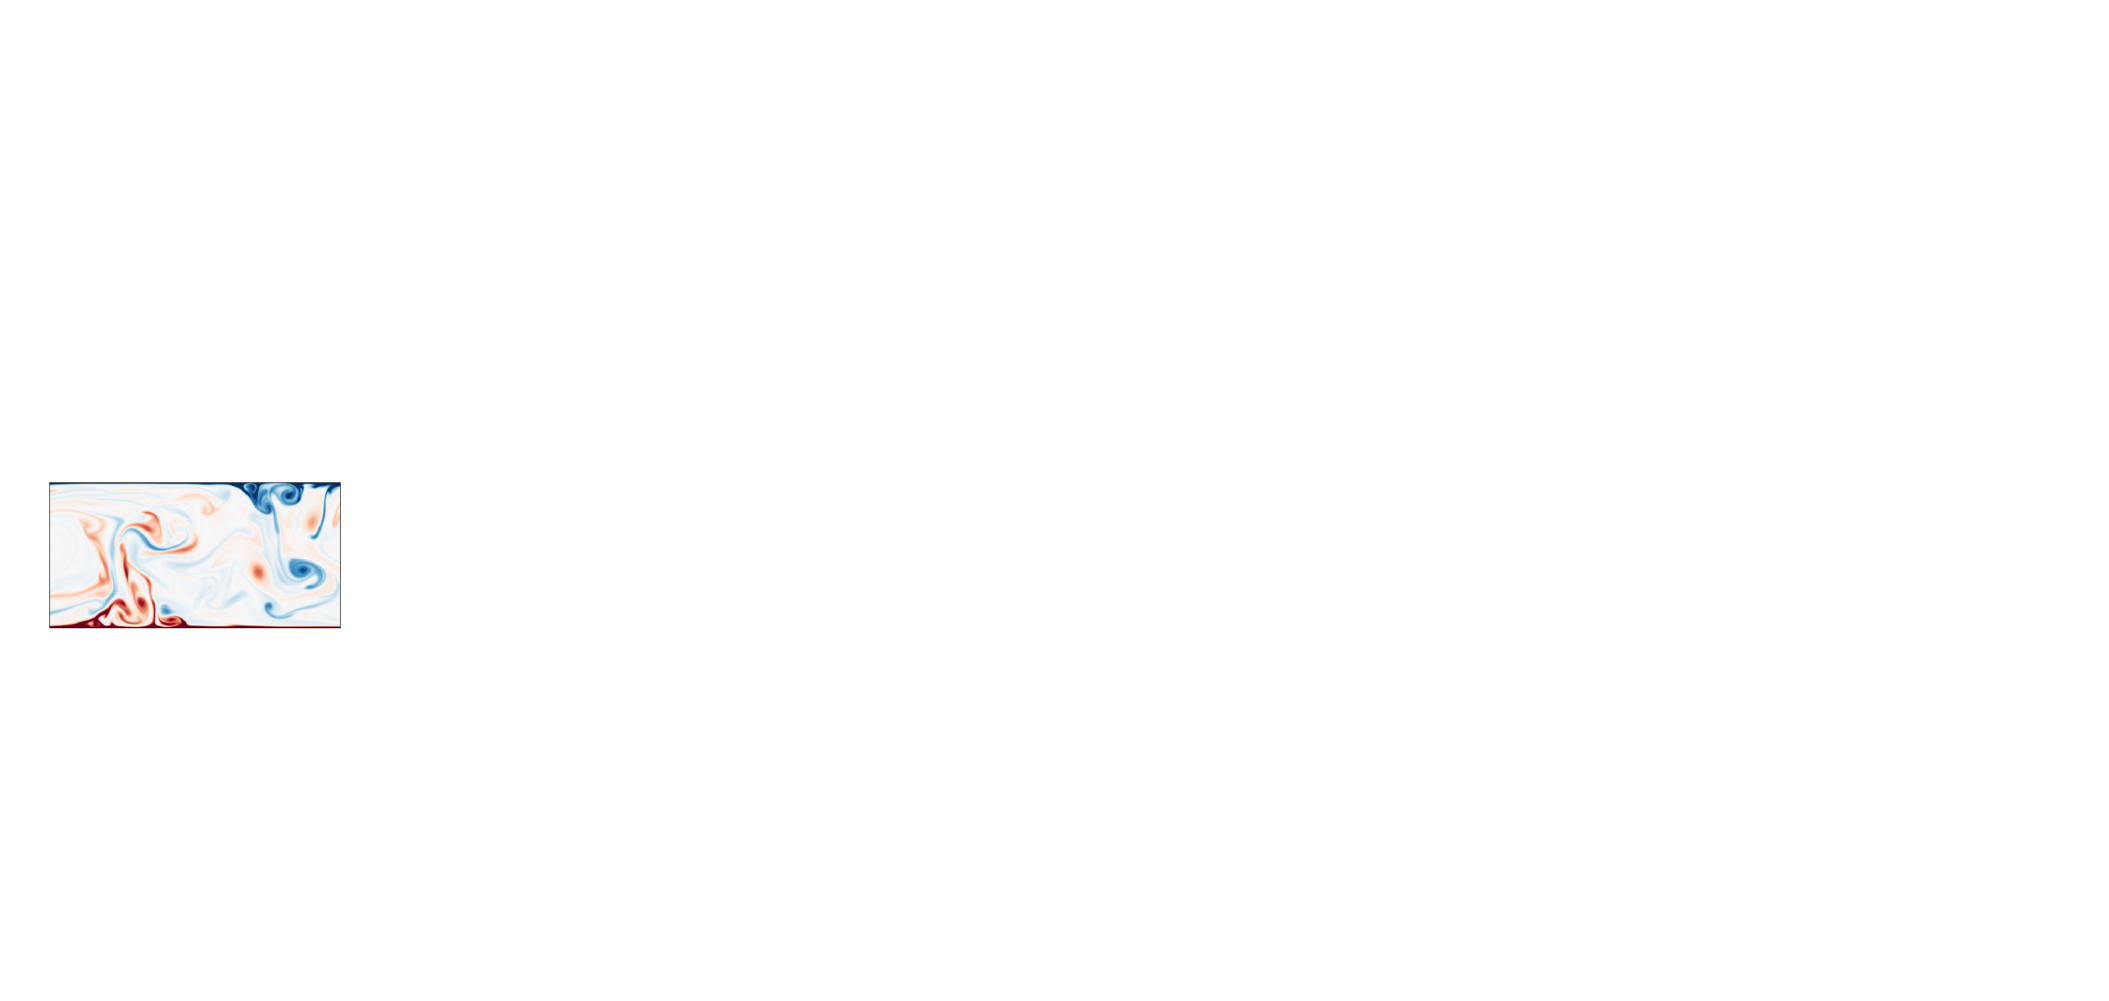
\includegraphics[width=\linewidth]{figures/method1.pdf}
\end{frame}

\begin{frame}
    \centering
    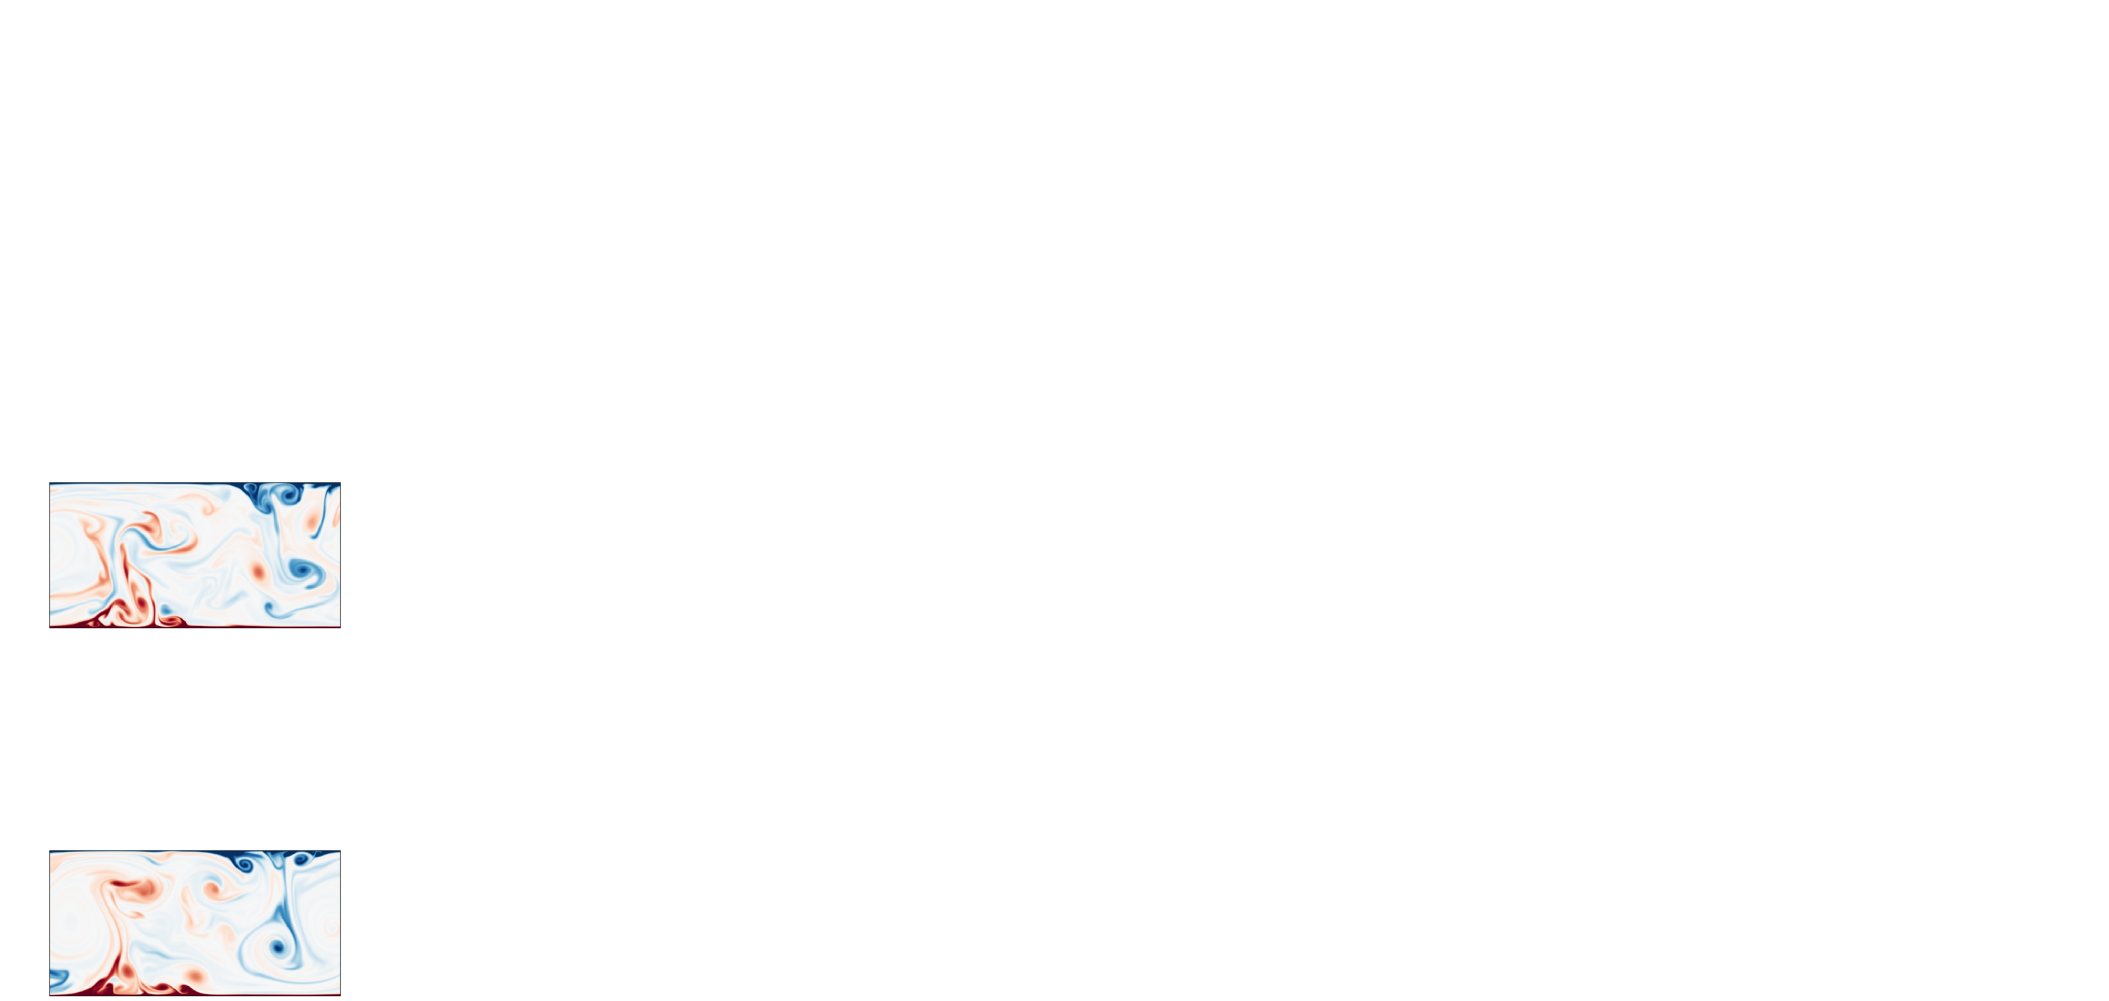
\includegraphics[width=\linewidth]{figures/method2.pdf}
\end{frame}

\begin{frame}
    \centering
    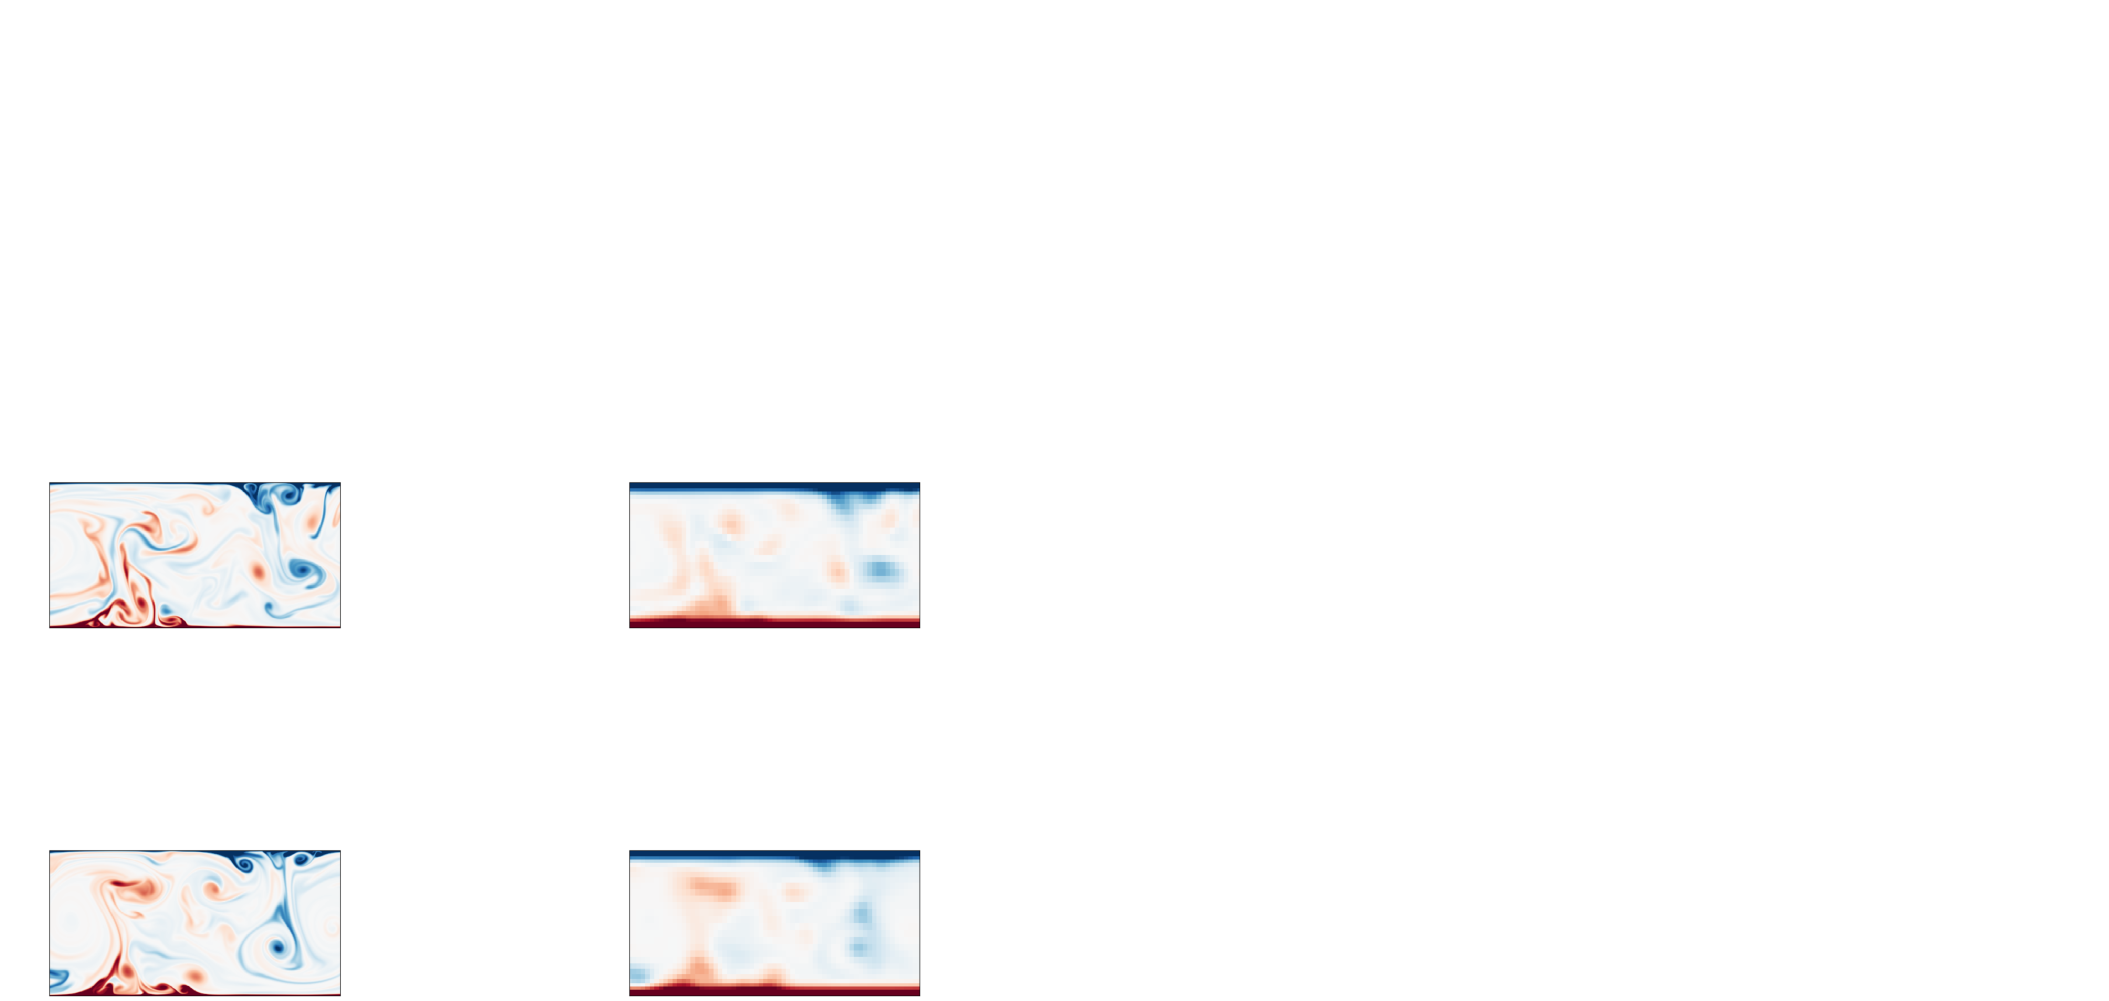
\includegraphics[width=\linewidth]{figures/method3.pdf}
\end{frame}

\begin{frame}
    \centering
    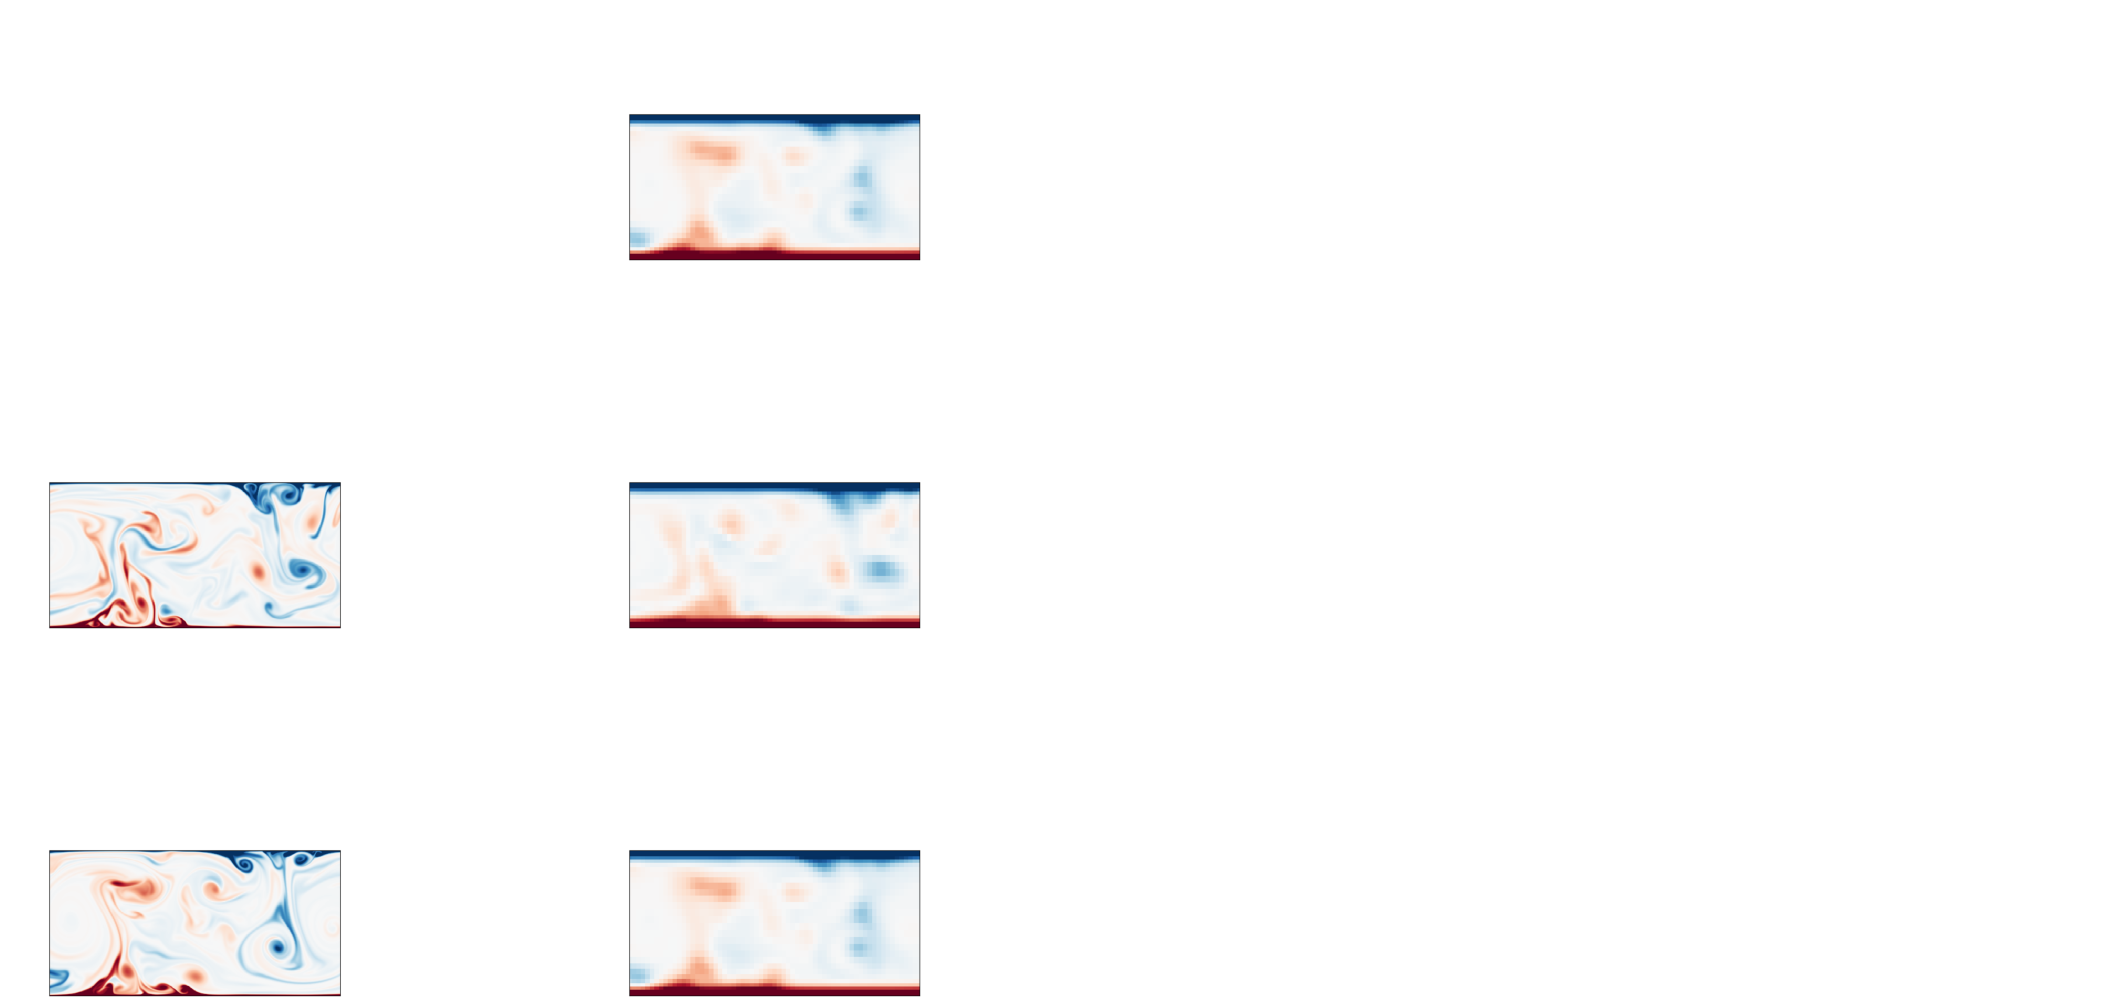
\includegraphics[width=\linewidth]{figures/method4.pdf}
\end{frame}

\begin{frame}
    \centering
    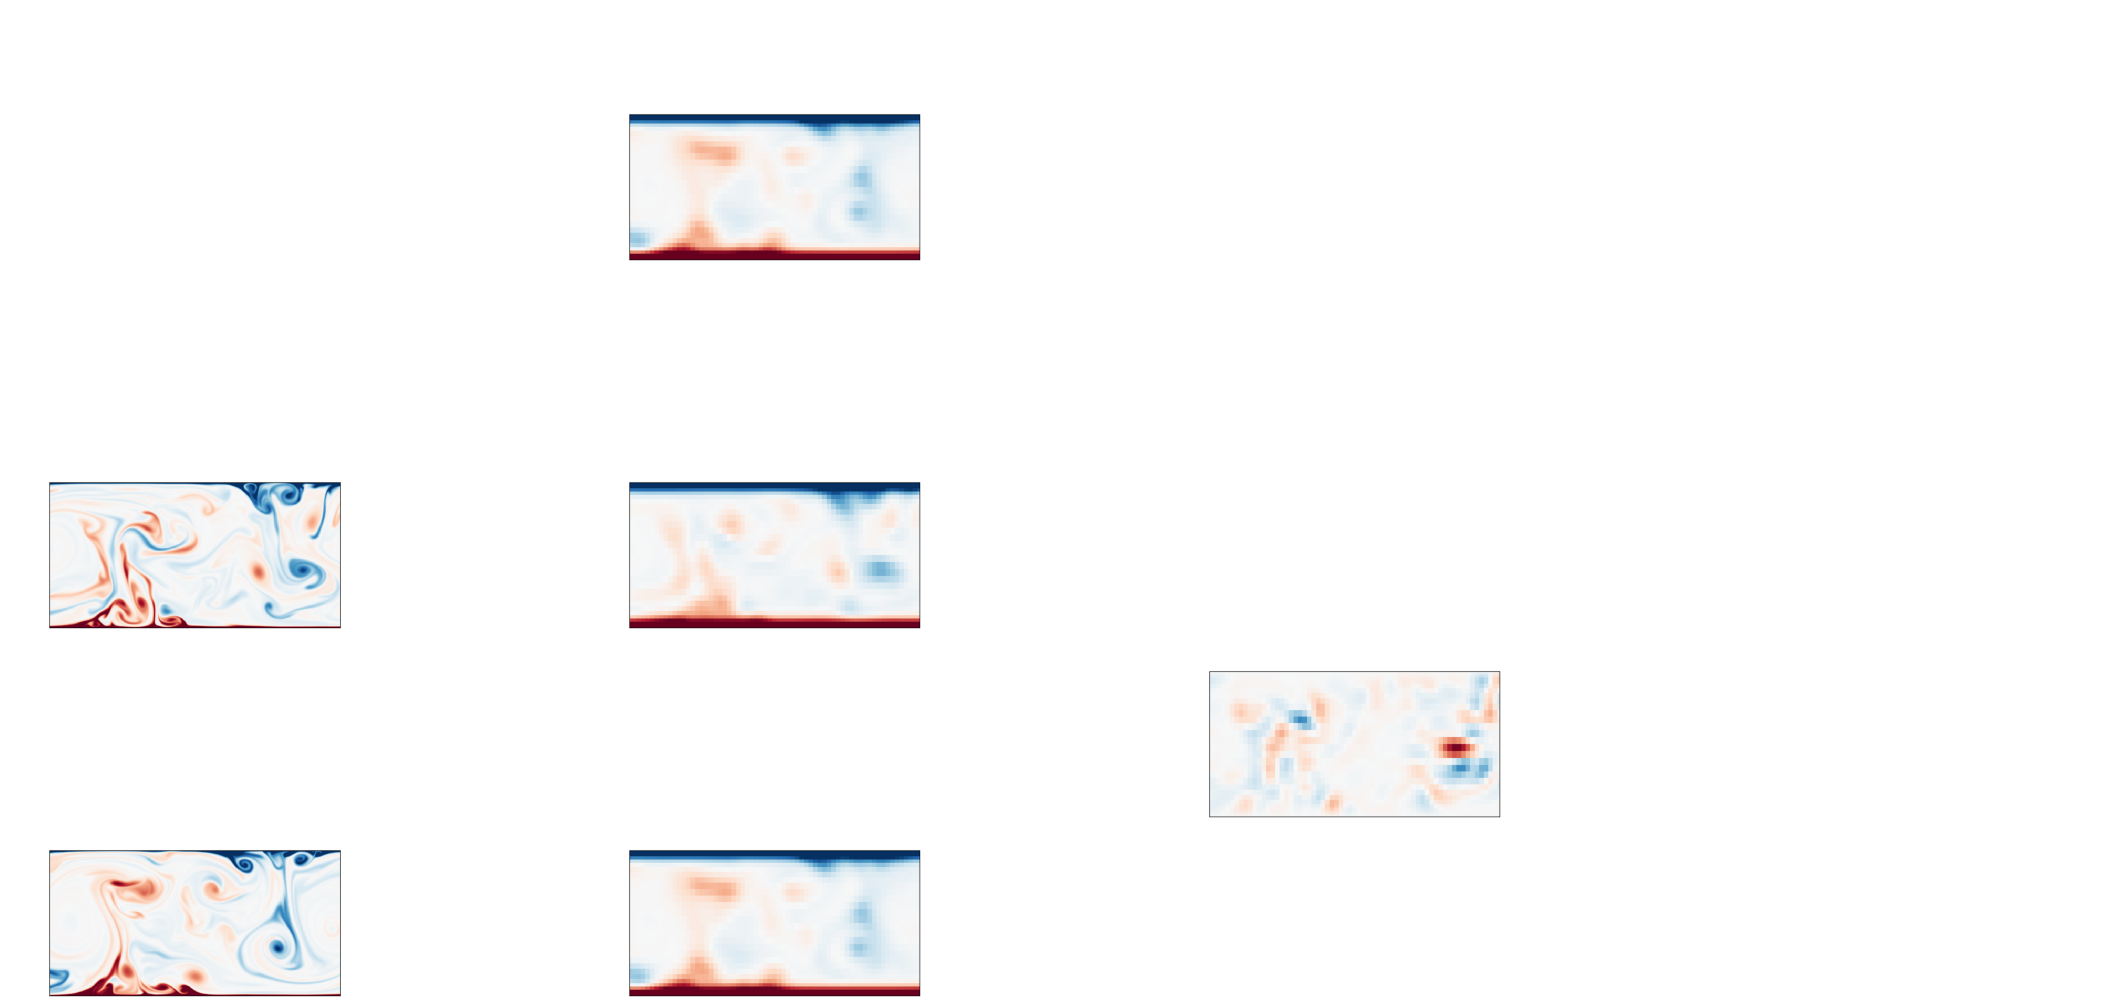
\includegraphics[width=\linewidth]{figures/method5.pdf}
\end{frame}

\begin{frame}
    \centering
    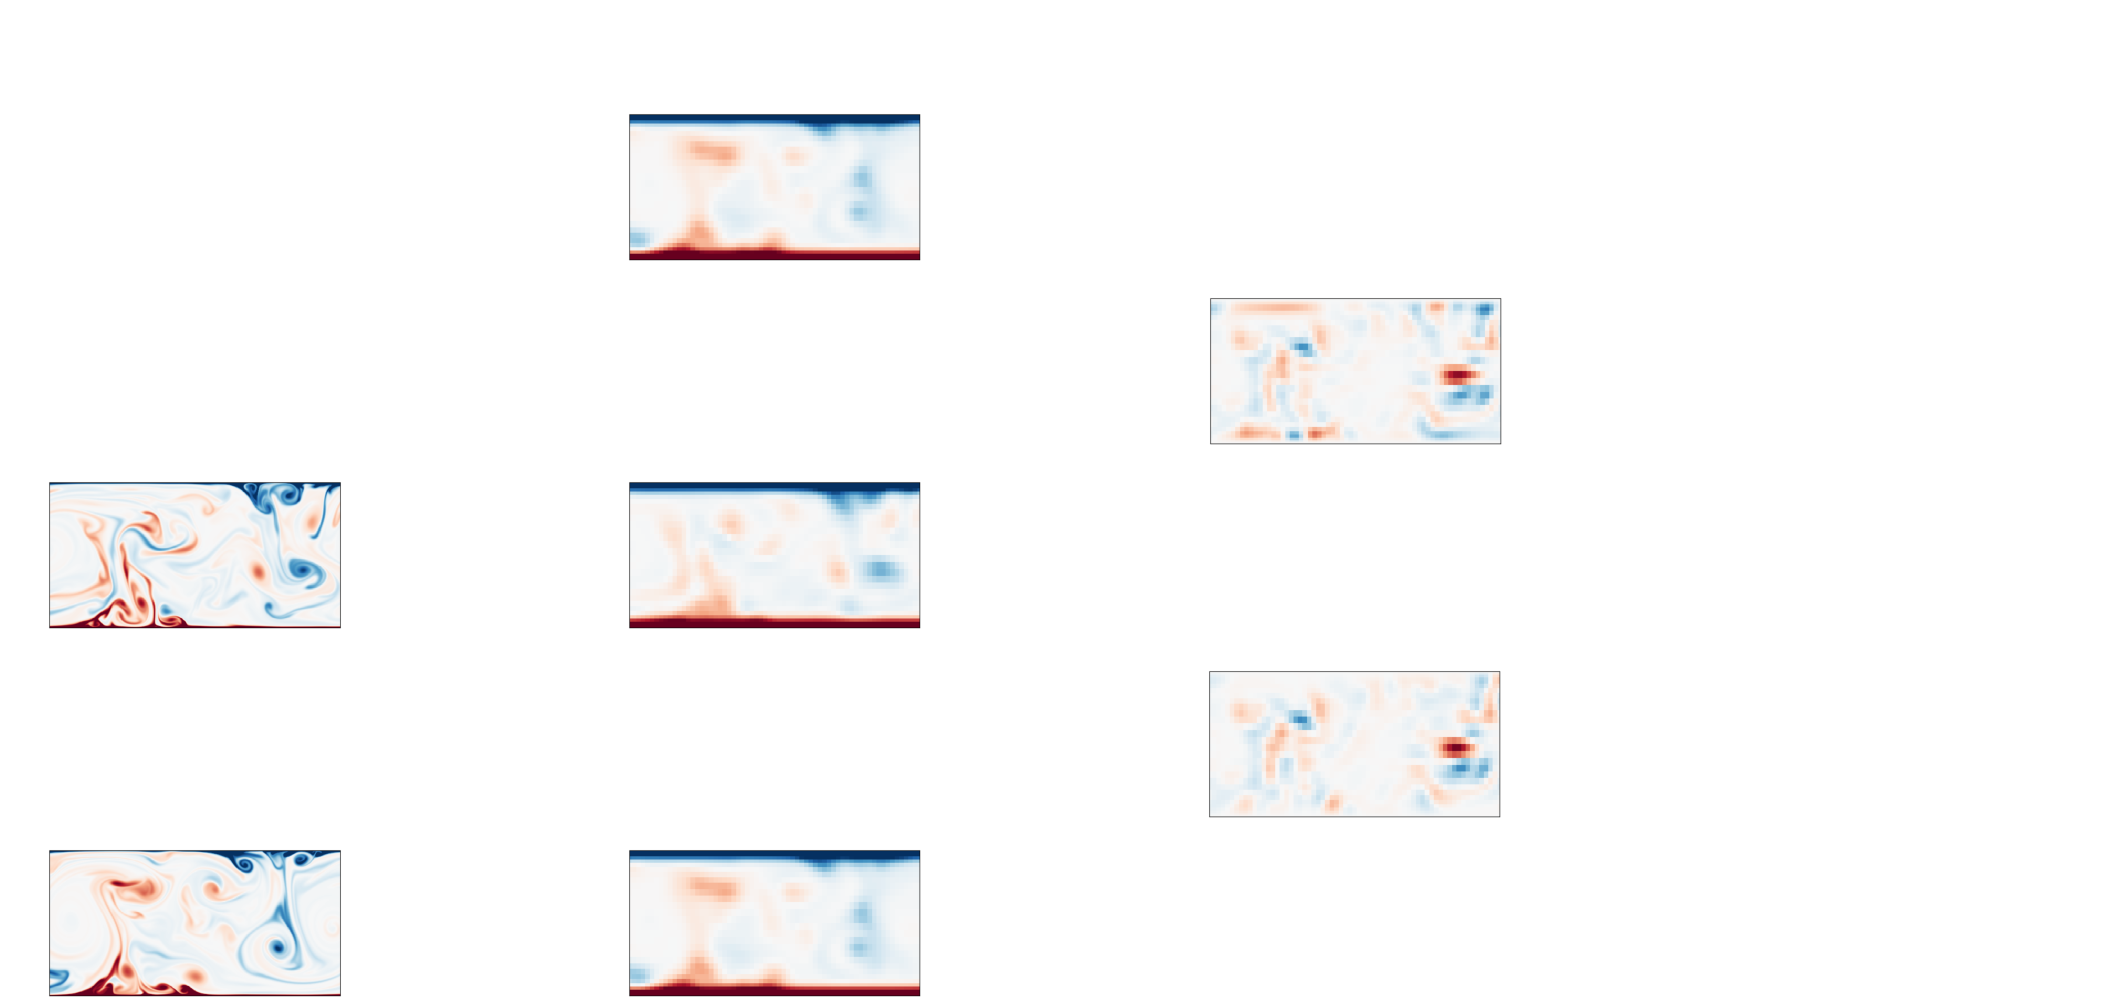
\includegraphics[width=\linewidth]{figures/method6.pdf}
\end{frame}

\begin{frame}
    \centering
    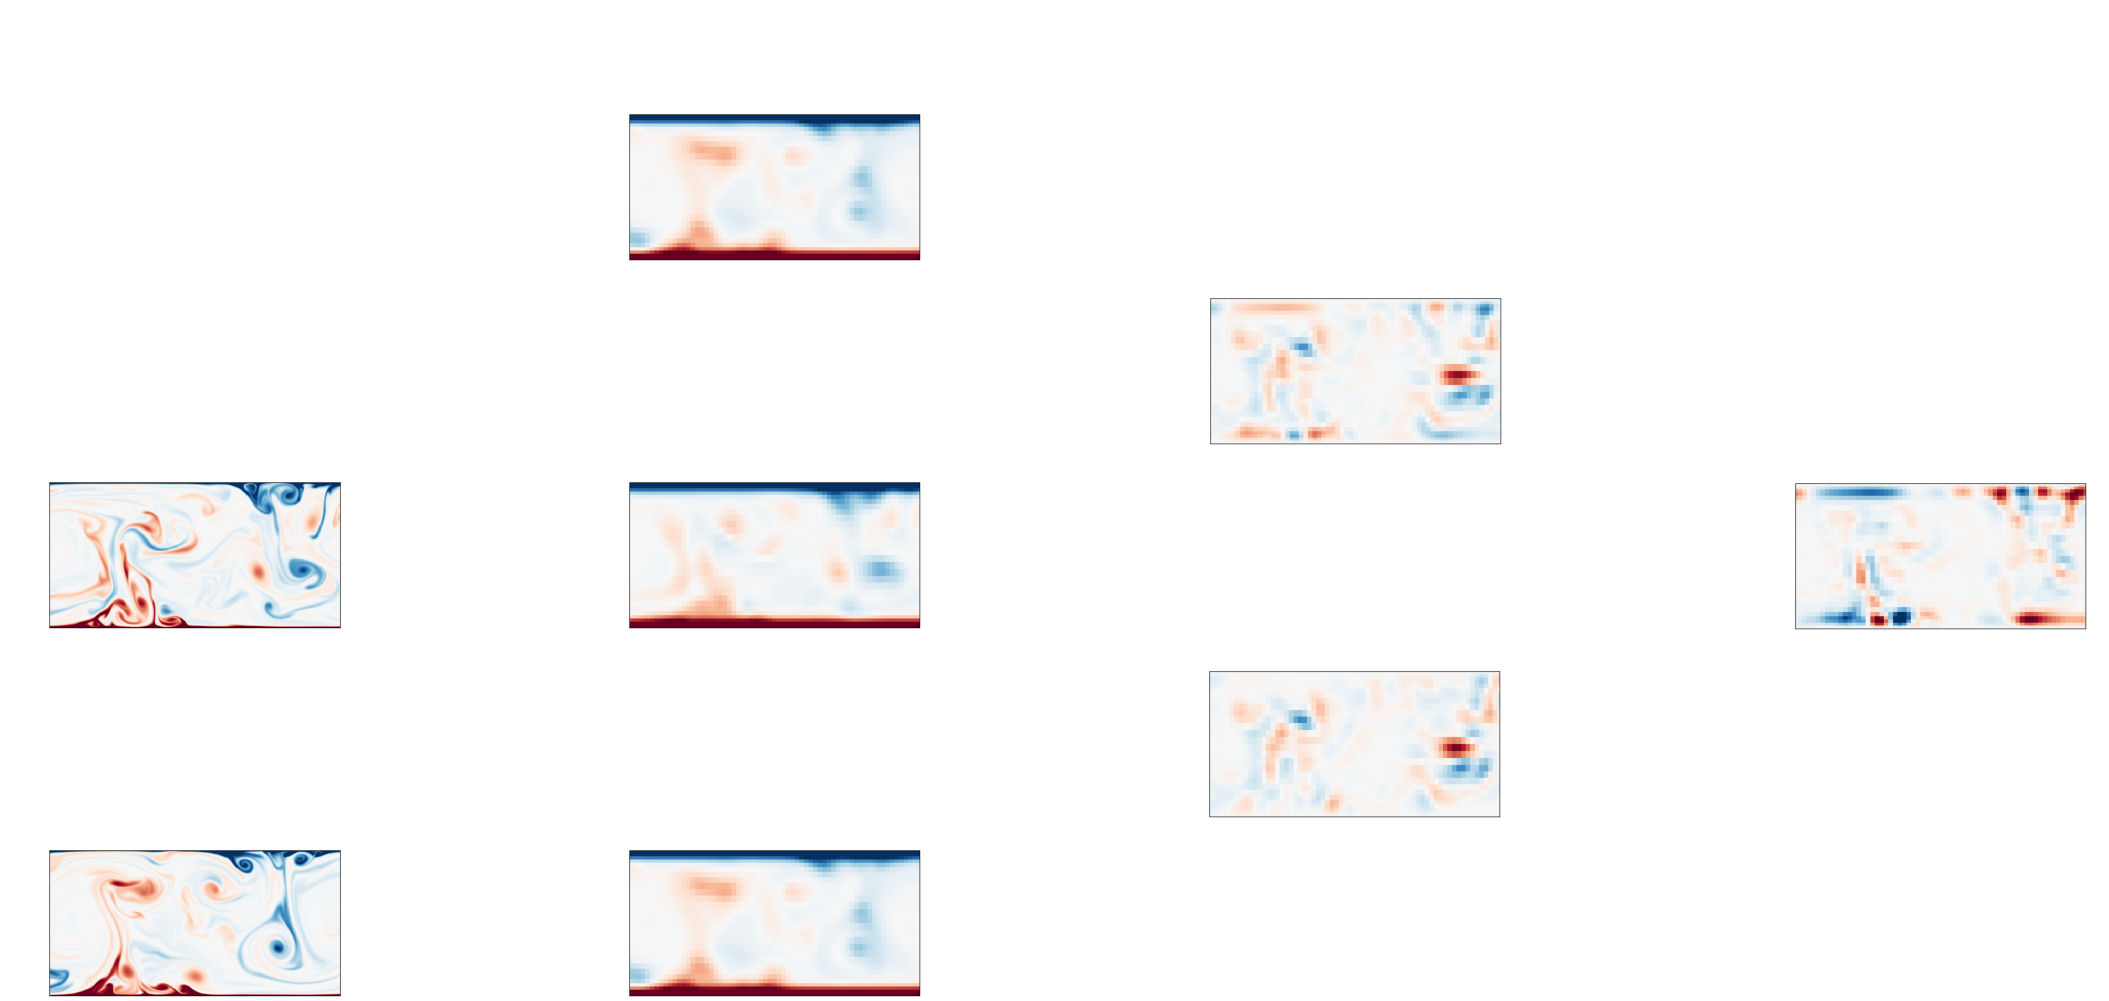
\includegraphics[width=\linewidth]{figures/method7.pdf}
\end{frame}

\begin{frame}
    \centering
    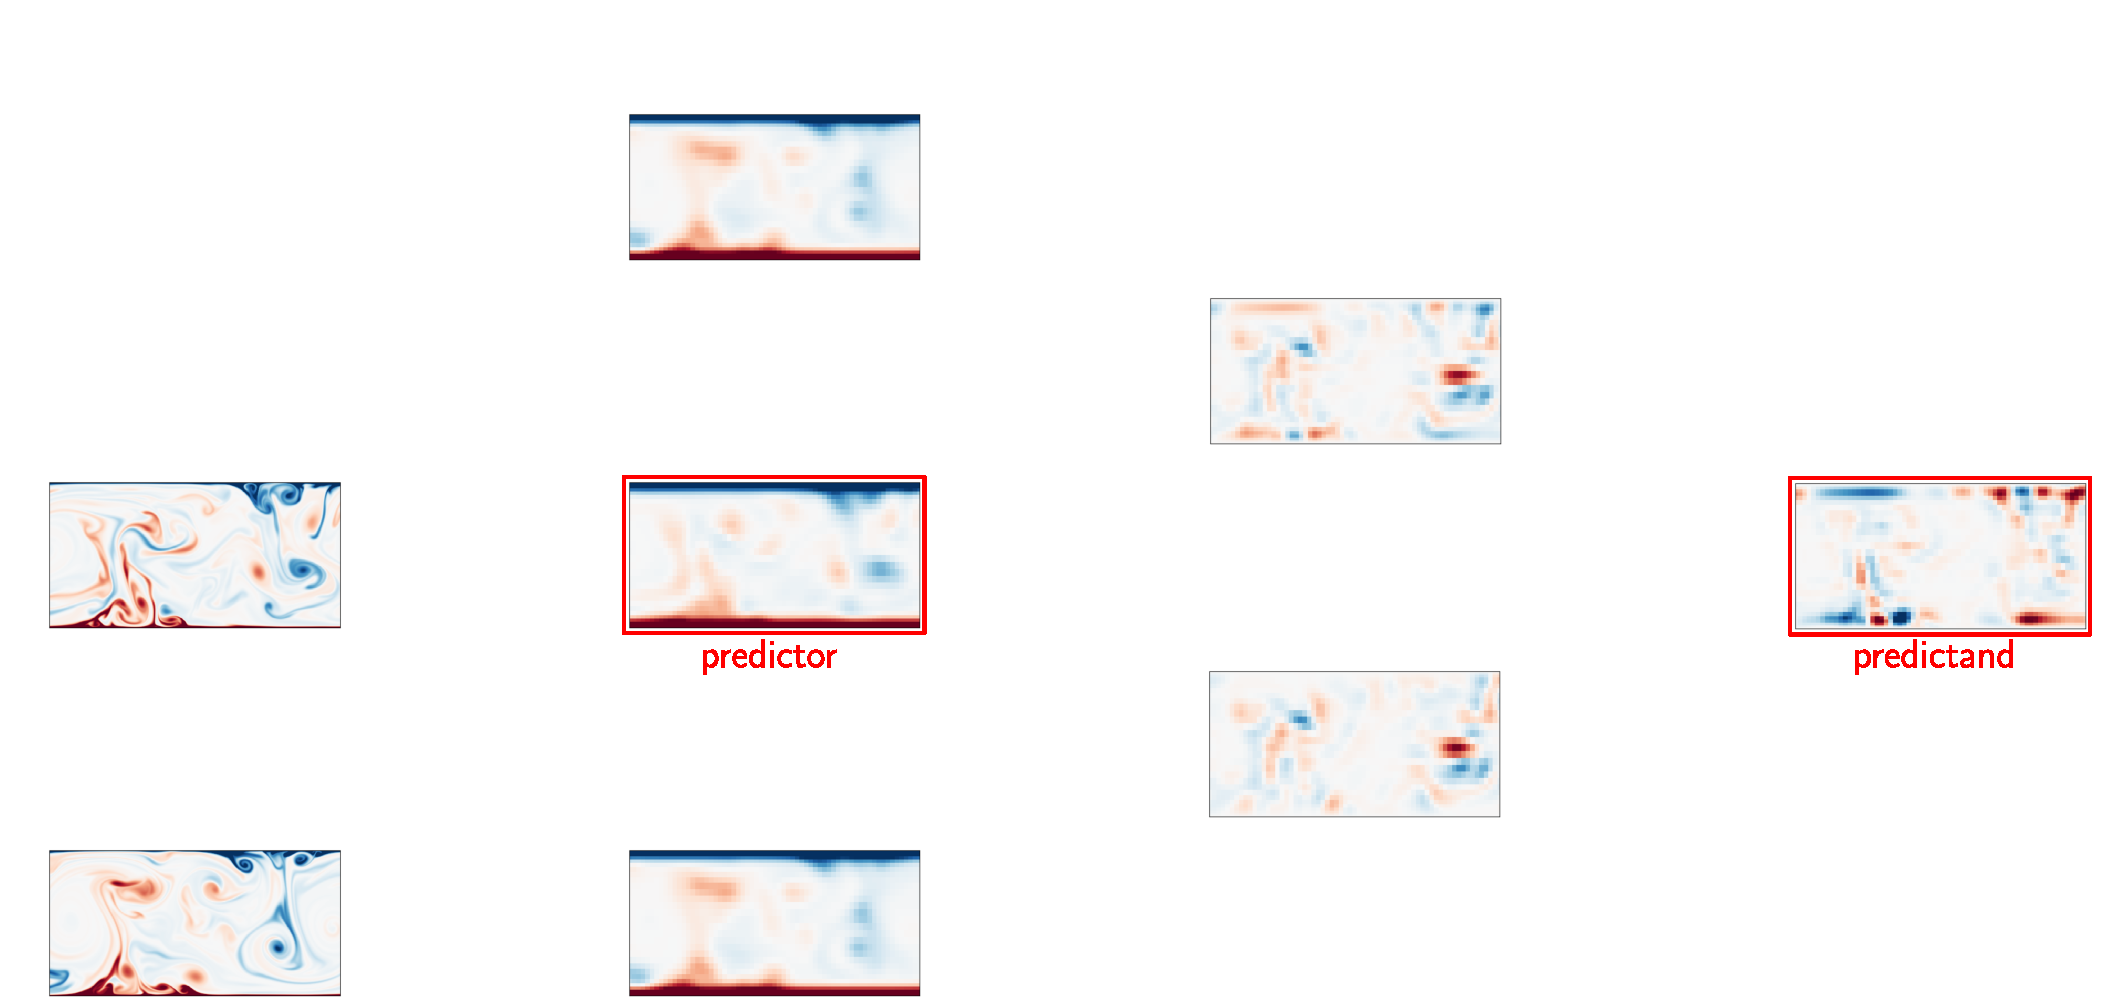
\includegraphics[width=\linewidth]{figures/method8.pdf}
\end{frame}

\begin{frame}
    \centering
    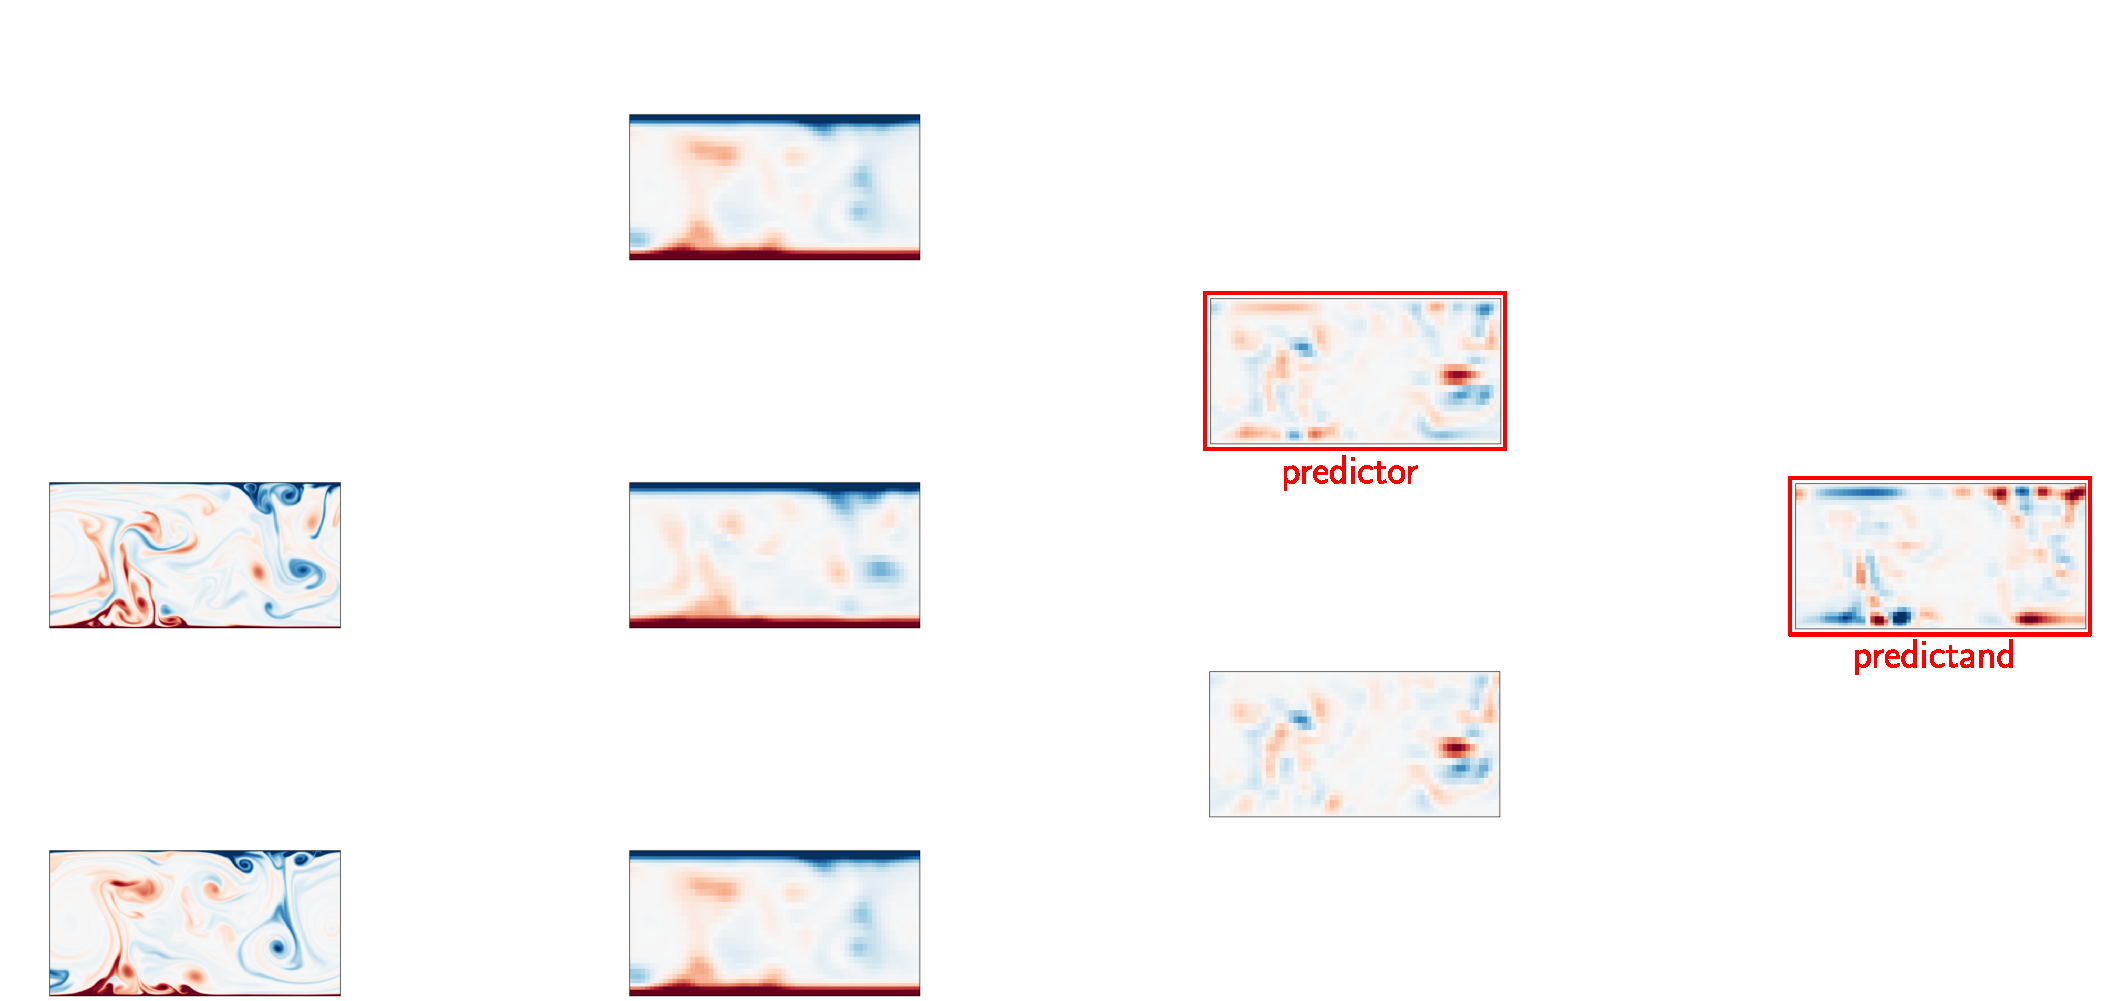
\includegraphics[width=\linewidth]{figures/method9.pdf}
\end{frame}

\begin{frame}
    \centering
    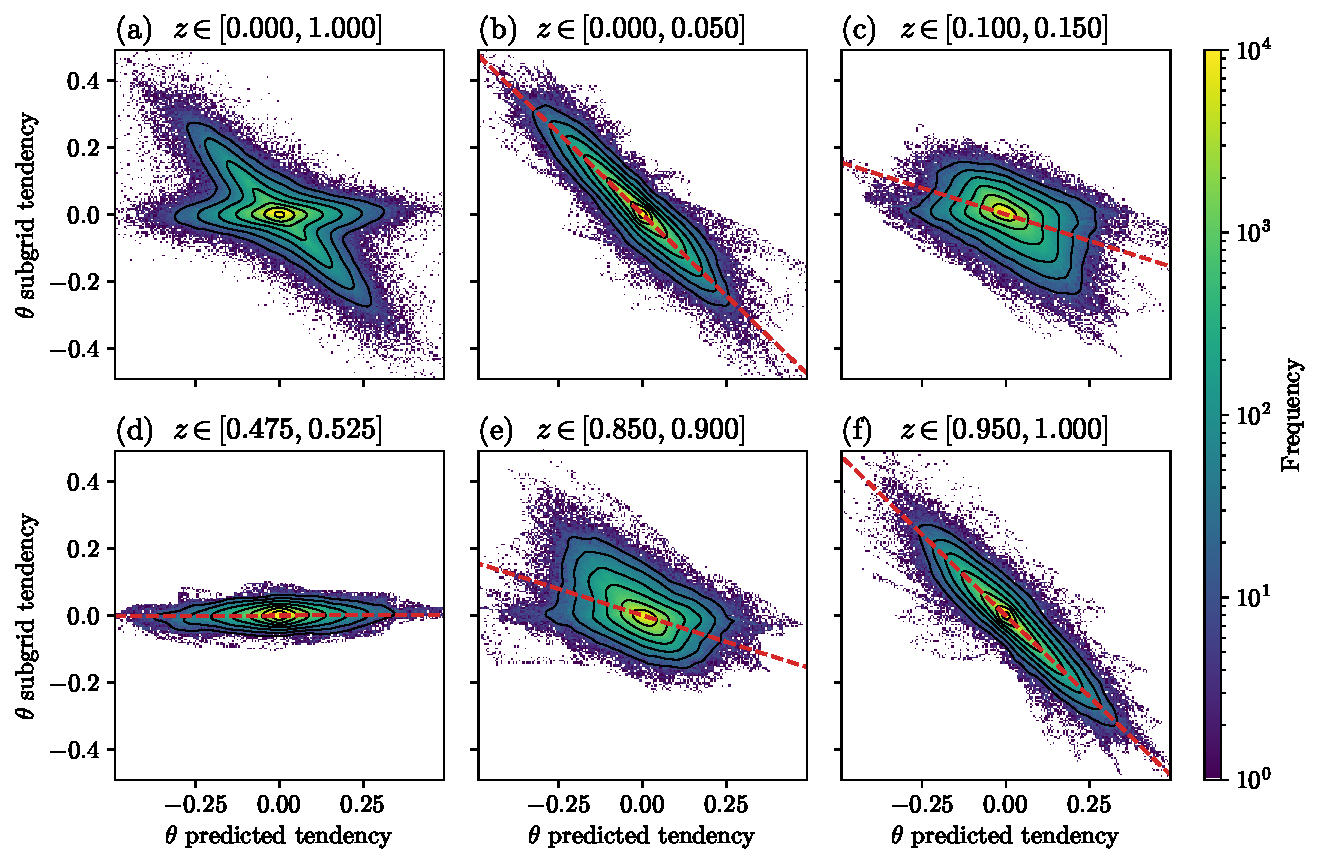
\includegraphics[height=0.99\textheight]{figures/theta_subgrid_vs_pred_tend.pdf}
\end{frame}

\begin{frame}
    \begin{align*}
        \pdiff{\vec{u}}{t} &= \cdots \\
        \pdiff{\theta}{t} &= \cdots \onslide<2>{\color{hilight} + \text{subgrid tendency model}}
    \end{align*}
\end{frame}

\begin{frame}
    \centering
    \begin{description}[align=right, labelwidth=0.5cm]
        \item[Truth] $2048 \times 256$, no forcing
        \item[Control]  $256 \times 64$, no forcing
        \item[Parametrised]  $256 \times 64$, with forcing
    \end{description}
\end{frame}

\begin{frame}
    \centering
    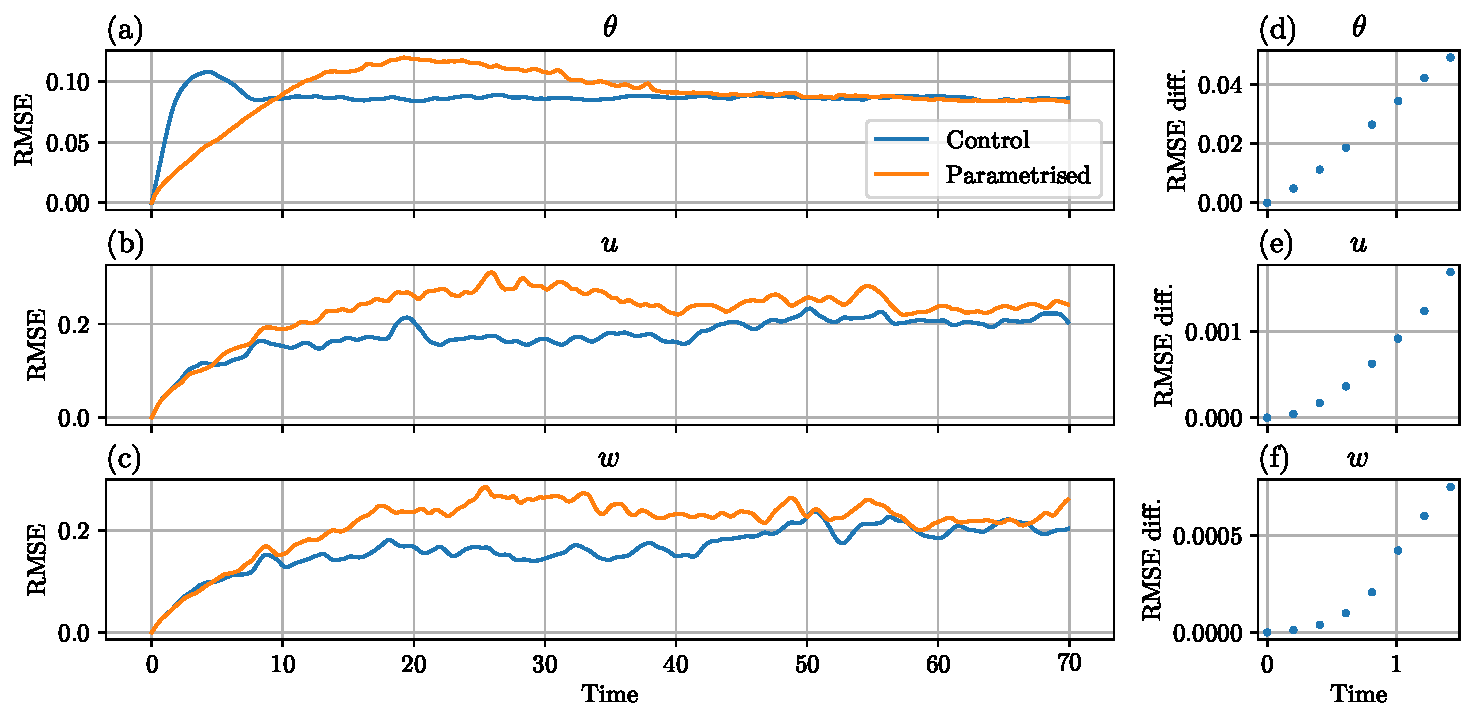
\includegraphics[width=\linewidth]{figures/rmse.pdf}
\end{frame}

\begin{frame}
    \centering
    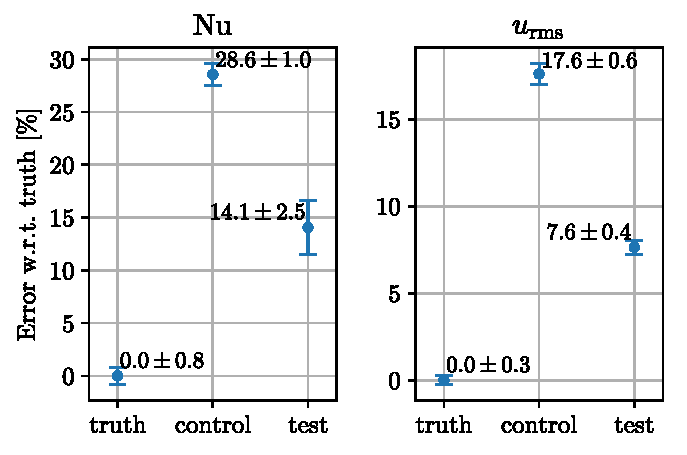
\includegraphics[height=0.99\textheight]{figures/stats.pdf}
\end{frame}

\begin{frame}
    \setbeamertemplate{enumerate items}[default]
    \begin{columns}
        \begin{column}{0.75\linewidth}
            \begin{itemize}
                \setlength{\itemsep}{6pt}
                \item Implemented a test bed for data-driven parametrisation
                \item Constructed a proof of concept by:
                \vspace{6pt}
                \begin{enumerate}
                    \setlength{\itemsep}{6pt}
                    \item Calculating subgrid tendencies
                    \item Fitting a statistical model to predict them
                    \item Using predicted subgrid tendencies to force
                        a coarse model
                    \item Demonstrating improved short-term forecast and
                        long-term statistical (``climate'') accuracy
                \end{enumerate}
                \item Future work: machine learning, stochasticity, memory
            \end{itemize}
        \end{column}
        \begin{column}{0.25\linewidth}
            \centering
            
\includegraphics[width=\linewidth]{figures/qr_code.pdf}
        \end{column}
    \end{columns}
\end{frame}

\end{document}
